%% This is free and unencumbered software released into the public domain.

%% Anyone is free to copy, modify, publish, use, compile, sell, or
%% distribute this software, either in source code form or as a compiled
%% binary, for any purpose, commercial or non-commercial, and by any
%% means.

%% In jurisdictions that recognize copyright laws, the author or authors
%% of this software dedicate any and all copyright interest in the
%% software to the public domain. We make this dedication for the benefit
%% of the public at large and to the detriment of our heirs and
%% successors. We intend this dedication to be an overt act of
%% relinquishment in perpetuity of all present and future rights to this
%% software under copyright law.

%% THE SOFTWARE IS PROVIDED "AS IS", WITHOUT WARRANTY OF ANY KIND,
%% EXPRESS OR IMPLIED, INCLUDING BUT NOT LIMITED TO THE WARRANTIES OF
%% MERCHANTABILITY, FITNESS FOR A PARTICULAR PURPOSE AND NONINFRINGEMENT.
%% IN NO EVENT SHALL THE AUTHORS BE LIABLE FOR ANY CLAIM, DAMAGES OR
%% OTHER LIABILITY, WHETHER IN AN ACTION OF CONTRACT, TORT OR OTHERWISE,
%% ARISING FROM, OUT OF OR IN CONNECTION WITH THE SOFTWARE OR THE USE OR
%% OTHER DEALINGS IN THE SOFTWARE.

%% For more information, please refer to <https://unlicense.org>
%%
\chapter{State of the Art}\label{stateofart}
Historically, at the beginning of integrating circuits, hardware development was
performed manually at the transistors level. In the early days, the circuits'
complexity was such that engineers could manually design the circuit's layout.
With the exponential growth predicted by G. Moore in 1965, the industry started
to experiment and develop new scalable ways of conducting hardware development.
Facing manual development limitations, hardware designers started describing
circuits functionalities independently from the manufacturing technology by
modeling them with Computer Aided Design (CAD) tools. While this approach was
faster and less error-prone, it could only be parallelized to a certain degree.
A breakthrough in digital design happened with the switch from CAD tools to
Hardware Description Languages.

Hardware Description Languages or (HDL) are a set of languages used to describe
a digital circuit's behavior before translating it to a target architecture.
Other than achieving an agnostic representation of the hardware, HDLs introduced
the possibility of modeling circuits at a higher level. This higher level of
abstractions allowed engineers to simulate the circuits behavior before
translating them to hardware. Similar to regular programming languages, HDLs are
composed of expressions and control structures, but contrary to standard
languages, each expression and control structure can be directly mapped to a
circuit behavior. VHDL and Verilog are the two most known and used HDL
standards. VHDL was initially developed by the U.S. Department of Defense
between 1983 and 1985. It is based on Ada programming language, and it became an
IEEE standard in 1987 \cite{coelho2012vhdl}. On the other hand, Verilog was
designed in the same period by Phil Moorby and Prabhu Goel as a hardware
description language based on the C language. Contrary to VHDL, Verilog was a
proprietary language that was bought by Cadence in 1989, which made it public in
1990 and finally became an IEEE standard in 1995 \cite{tala2003verilog}.

While from the middle 1980s, integrated circuits made enormous leaps forward
year by year, the leading technologies used to describe the integrated circuits
are still VHDL and Verilog. The new revision of the standards came along for
Verilog in 2005 and VHDL 2008. These last two standards are focused on stability
and clarifications rather than new features.

In the last few years, these legacy HDL have aged rapidly. Deriving from old
languages like Ada and C makes them lacking the expressiveness of modern
languages, leading to low re-usability of components across different designs
and reducing designer productivity \cite{bachrach2012chisel}. Creating efficient
hardware requires the designer to rapidly explore different designs and
architecture, which is unmanageable with traditional HDL given their poor
re-usability. Many attempts were made to circumvent the legacy languages'
limitations by using other languages like Perl \cite{shacham2012avoiding} or
Scheme \cite{jennings1999verischemelog} to pre-process scripts and macros to
enable parametric hardware generations. This approach is not ideal because the
companion language used to achieve this flexibility is not syntactically aware
of the hardware language, leading to unsound hardware generation and increased
maintenance work.

Parallel to the design limitations offered by traditional HDLs, their language
capabilities are not suitable for the verification process. This process,
described in-depth in the next chapters, requires high-level constructs not
available in common HDLs. As for hardware design, to overcome these limitations,
companies started developing separated languages meant only to verify the
hardware model described in Verilog and VHDL \cite{edwards2004design}. This
difference in the language used by the verification team and the design team
frequently creates a barrier of communication between the two teams, which
results in an overall delay in the development process. The following sections
explain how these problems were solved by two different languages, SystemVerilog
and Chisel, and how other companies rely on new tools for their verification
environment.

\section{SystemVerilog}
For many years, Verilog's and VHDL's features offered engineers enough power to
model the hardware and create robust enough test benches to verify the model's
functionality. The advancements of silicon technology gave more opportunities to
create larger designs, and consequently, the number of lines needed for modeling
modern integrated circuits increased. This amount of code leads to a significant
increase in verification time required to verify chip designs. To solve the
intrinsic limitations of Verilog in the design and verification context and to
unify the two, the Accelera organization, in collaboration with the most
prominent representative from the EDA industry \cite{sutherland2003overview},
developed a new standard extending the Verilog 2001 one. Accelera, rather than
creating an entirely new language, defined a set of high-level extensions to
Verilog by combining and carefully reviewing technology donations from
Co-Desing, Synopsys, and many more. Further, it ensured that all SystemVerilog
enhancements were fully backward compatible with the Verilog language, which
implies that all existing Verilog models work with software tools that implement
the SystemVerilog standard.

Since the enhancements introduced by this new standard are an extension of the
Verilog language, they are parallel and categorized into two different groups,
Design enhancements and Verification additions, as shown in figure
\ref{fig:stoa:svcomponents}. Given the dual-nature of the language,
SystemVerilog is also referred to as the first HDVL, or Hardware Design
Verification Language.



\begin{figure}[htbp]
\centering
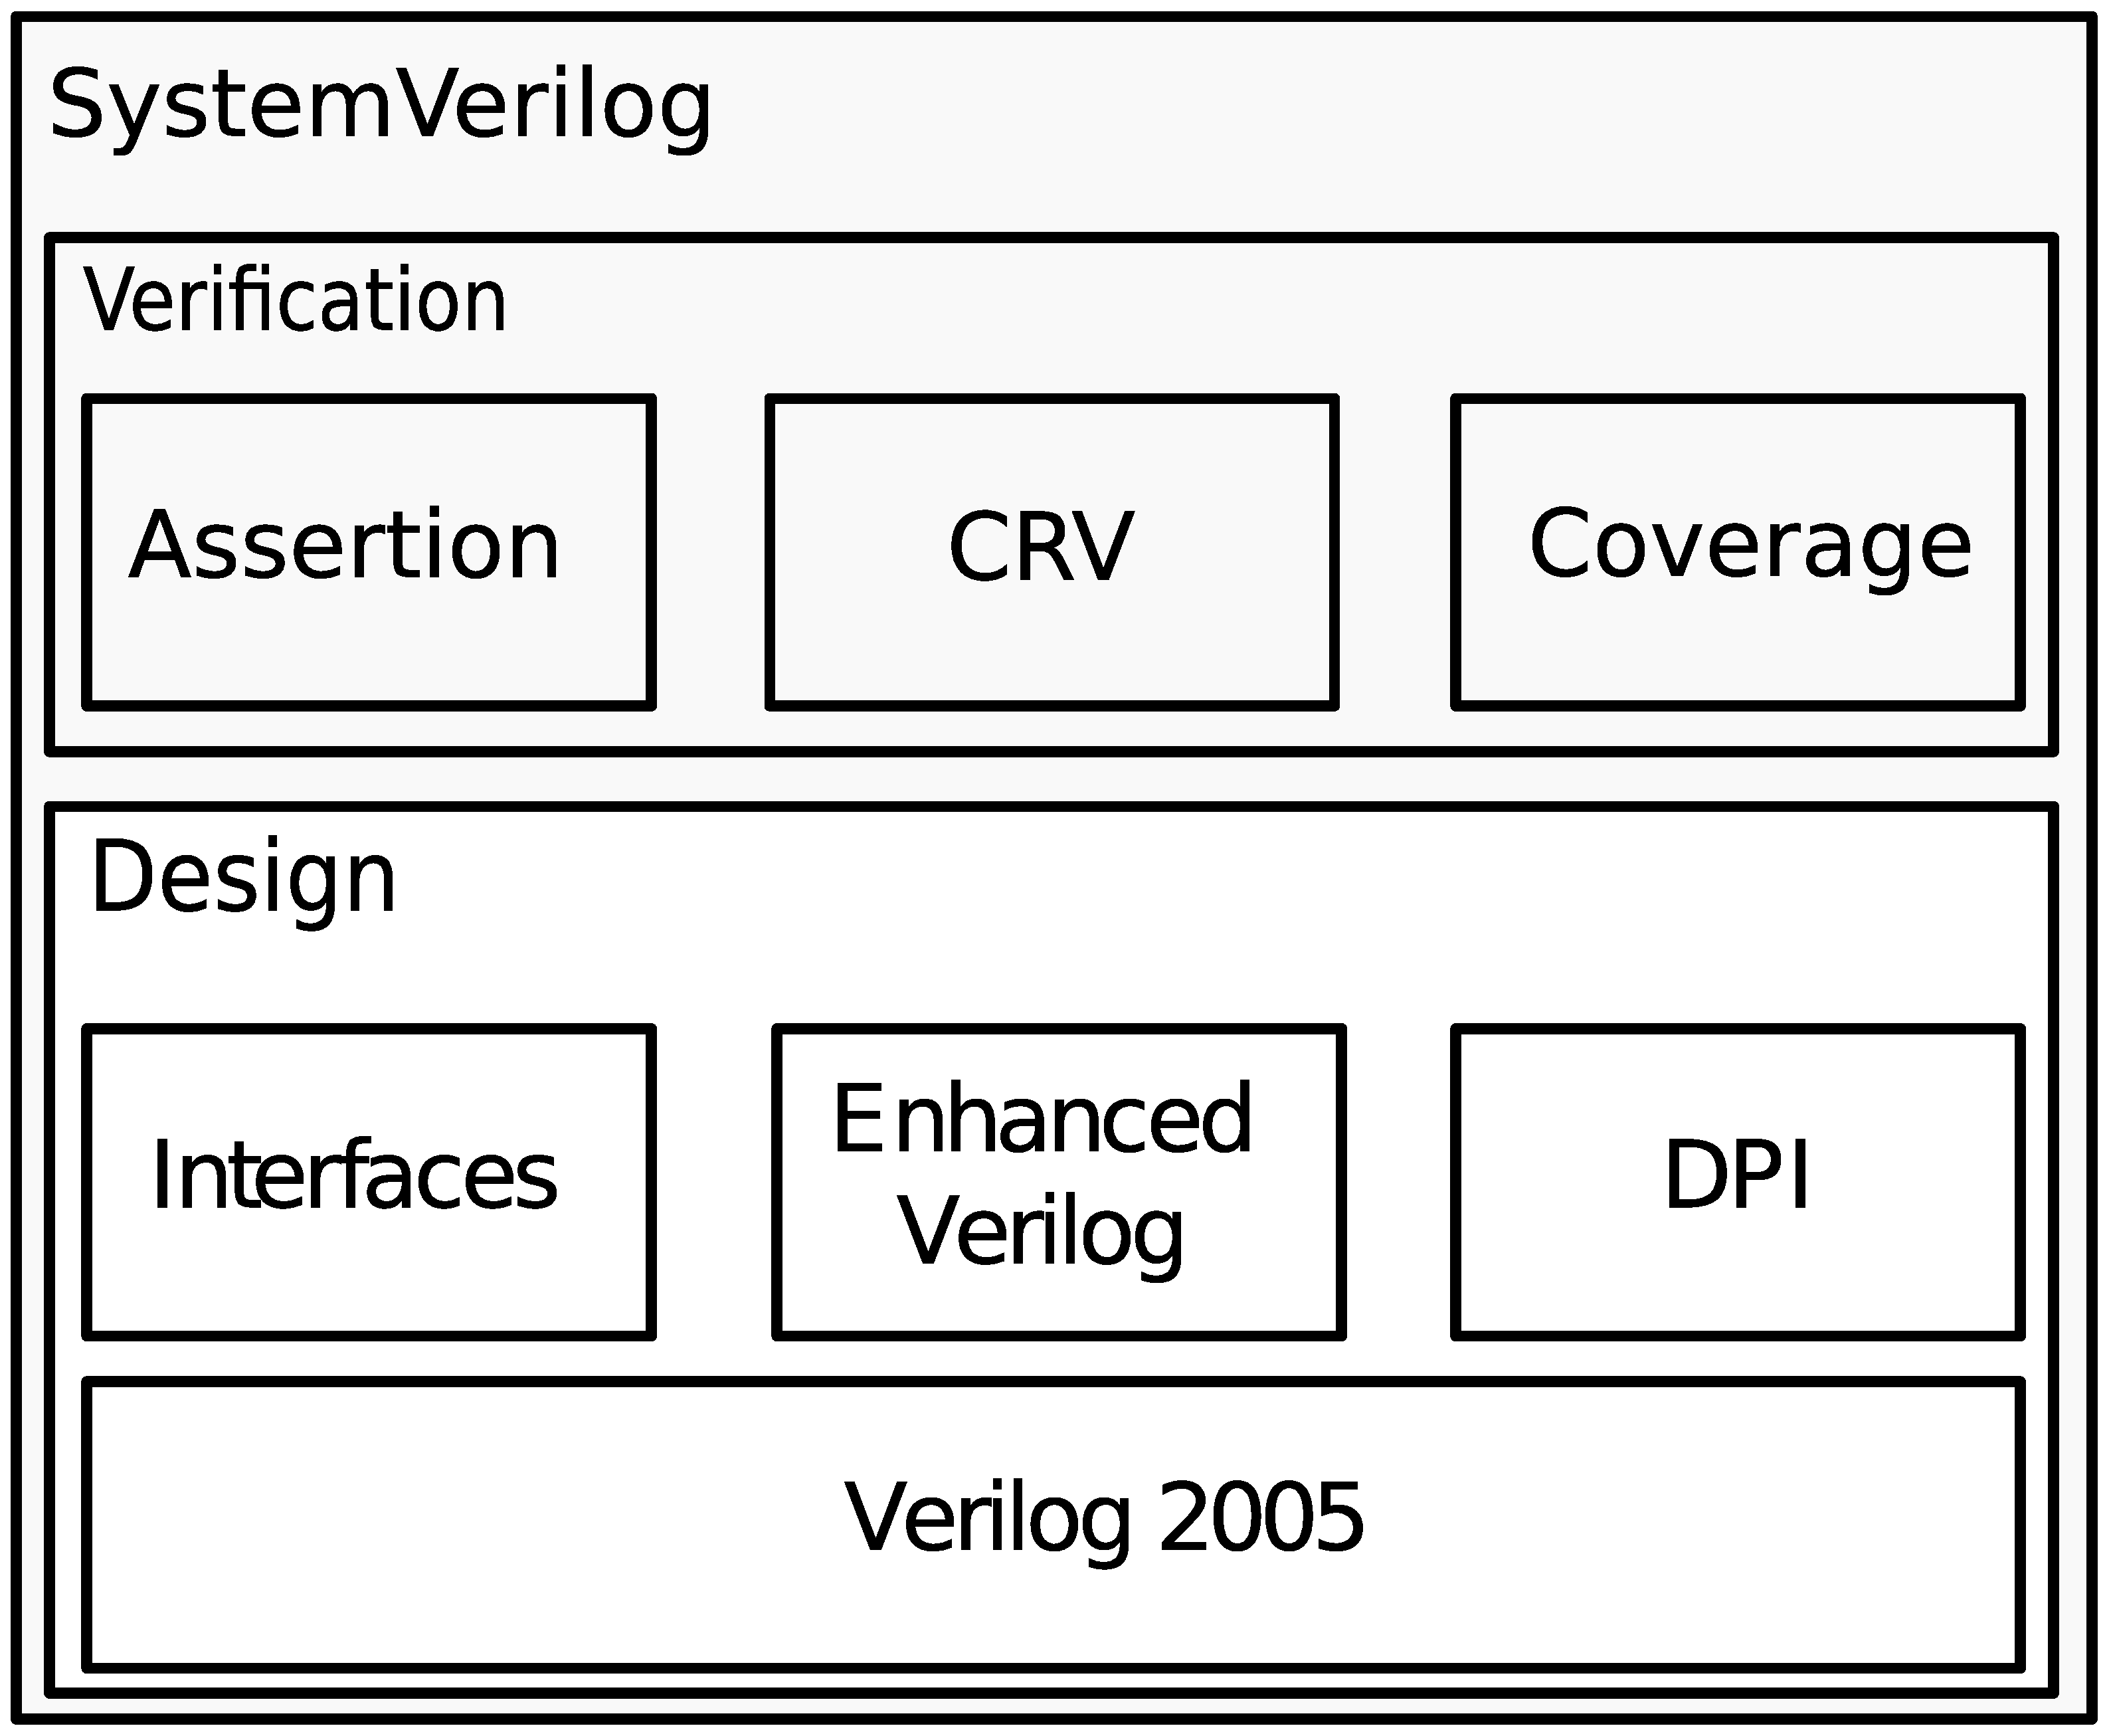
\includegraphics[width=0.5\linewidth]{pictures/SystemVerilog_structure.eps}
\caption{SystemVerilog language components \cite{rich2003evolution}.}
\label{fig:stoa:svcomponents}
\end{figure}

Below are reported some of the enhancements introduced by SystemVerilog

\begin{description}
    \item[Assertions] An assertion states that a specific condition, or sequence
      of conditions, in a design is correct. If the condition or sequence is not
      valid, the assertion statement will generate an error message.
      Furthermore, assertions can test for a condition or a sequence of
      conditions realized in multiple clock cycles. SystemVerilog assertions can
      be combined with functions in order to check complicated protocols value.
      Focusing on backward compatibility, SystemVerilog assertions can be
      defined outside of Verilog modules and bind them inside the verification
      environment to a specific module or module instance. This allows
      verification engineers to add assertions to existing Verilog models
      without changing the model.
    
    \item[Interfaces] SystemVerilog interfaces provide a new, high-level
      paradigm for modeling abstraction. Interfaces are used to simplify the
      modeling and verification of large and intricate designs. This new
      construct was added to the language to encapsulate the communication
      between blocks allowing the engineers to avoid the duplicated declaration
      of module ports. An interface is defined using the new keywords
      ``interface” and ``endinterface.” SystemVerilog modules can use an
      interface as a single port representing a bundle of wires. Other than
      representing a bundle of wires, interfaces can include standard
      functionality that can be used across all the modules implementing the
      specific interface. For example, an Interface can have a built-in protocol
      checking \cite{sutherland2003overview}.
    
    \item[Classes] SystemVerilog introduces the Object-Oriented Programming
      paradigm by \hfill \break adding objects and classes to the Verilog
      language, similar to Java and C++. A class is a container for data
      declarations and methods operating on the data itself, which also enables
      polymorphism through inheritance. Like in Java, SystemVerilog manages the
      memory allocation and provides a garbage collector to prevent memory
      leaks. Given the dynamic nature of classes, the SV standard does not allow
      the synthesis of classes, and thus this feature is only inside the
      simulation environment.
    
    \item[CRV] Like most programming languages, Verilog HDL includes basic
      random number generator functionalities. As explained further in the
      document, this function gives weak control over the random sequence
      generation. Thanks to its OOP (Object-Oriented Programming) paradigm,
      SystemVerilog revolutionizes the generation of random sequences by
      allowing the creation of random objects. In SV, classes can declare random
      fields using two new keywords, ``rand" and ``randc." These fields can then
      be constrained using functions that state the possible values that these
      fields can have. This allows the verification engineers to create ad hoc
      sequences of vectors that specifically test the desired functionalities.
      Constrained random testing and coverage driven verification are explained
      more in-depth in the latter part of the report.
    
    \item[Coverage] SystemVerilog embedded functional coverage inside the
      language specifications by introducing two types of functional coverage.
      The first flavor leverage the same syntax used by SystemVerilog assertions
      to specify the cover specifications applied to a model's properties and
      sequences. This allows the design engineer to use the property to collect
      functional coverage and assertion with the disadvantages that these cover
      properties can be applied only to structural code and not used inside
      class-based objects. The second flavor of functional coverage is the
      so-called cover-groups. Cover-groups are used to track the number of
      occurrences of a value specified as an instance of a cover-point and can
      be used in structural and class-based objects.
    
    \item[Direct Programming Interface] One of the advancements in SystemVerilog
      is the introduction of the DPI interface. The DPI interface is a new means
      of interaction between functions written in C or C++ and SystemVerilog
      code without a complicated interface such as the Verilog Programming
      Language Interface. Values can be passed between the two languages
      allowing the verification engineers to test the simulation results
      directly against a golden model written in C or C++.

\end{description}
SystemVerilog aimed to be a single language sufficient to express and model
digital systems at various abstraction levels, from untimed functional models to
RTL design. Despite its richness, it became clear during the early adoption of
the language that companies and verification engineers started to develop and
model the verification environment without following precise guidelines.
Although the language provided all the tools needed to implement a rich
verification environment, the language complexity caused confusion and practical
challenges among the verification engineers \cite{bromley2013if}. This led to
the development of different methodologies before settling on to what is known
today as UVM or Universal Verification Methodology. The next section introduces
UVM, the leading verification methodology used by SystemVerilog engineers to
develop reusable verification components.

\section{UVM} \label{sec:uvm}
Given the SystemVerilog language's extensiveness, the vendor tools did not
support the full language set for quite some time after the specifications'
release, and each implementation provided a somewhat different subset of the
language. These differences in the features available led to the development of
different coding style between verification engineers based on the tools they
used. To overcome this disparity a decade ago, Accellera started creating an
open standard methodology compatible with all major vendors' tools. This effort
resulted in the creation of UVM.

\par UVM is a complete verification methodology that unites the best practices
for efficient and exhaustive digital design verification
\cite{methodology20111}. It leverages the OOP nature of System Verilog to create
UVM Verification Components or UVC, which are a set of classes reusable across
different projects and testbenches. The deciding aspects of UVM are the
open-source nature and the vast compatibility with all the vendor's tools. UVM
is provided as an open-source library that can be downloaded from the Accelera
website. Since UVM is based on SystemVerilog, it is possible to use UVM with any
simulator compatible with the SystemVerilog standard. The final goal of UVM is
to help the system engineers and verification engineers find bugs earlier in the
design process while providing a set of primitives and portable rules across
different simulators.

\begin{figure}[htb]
\centering
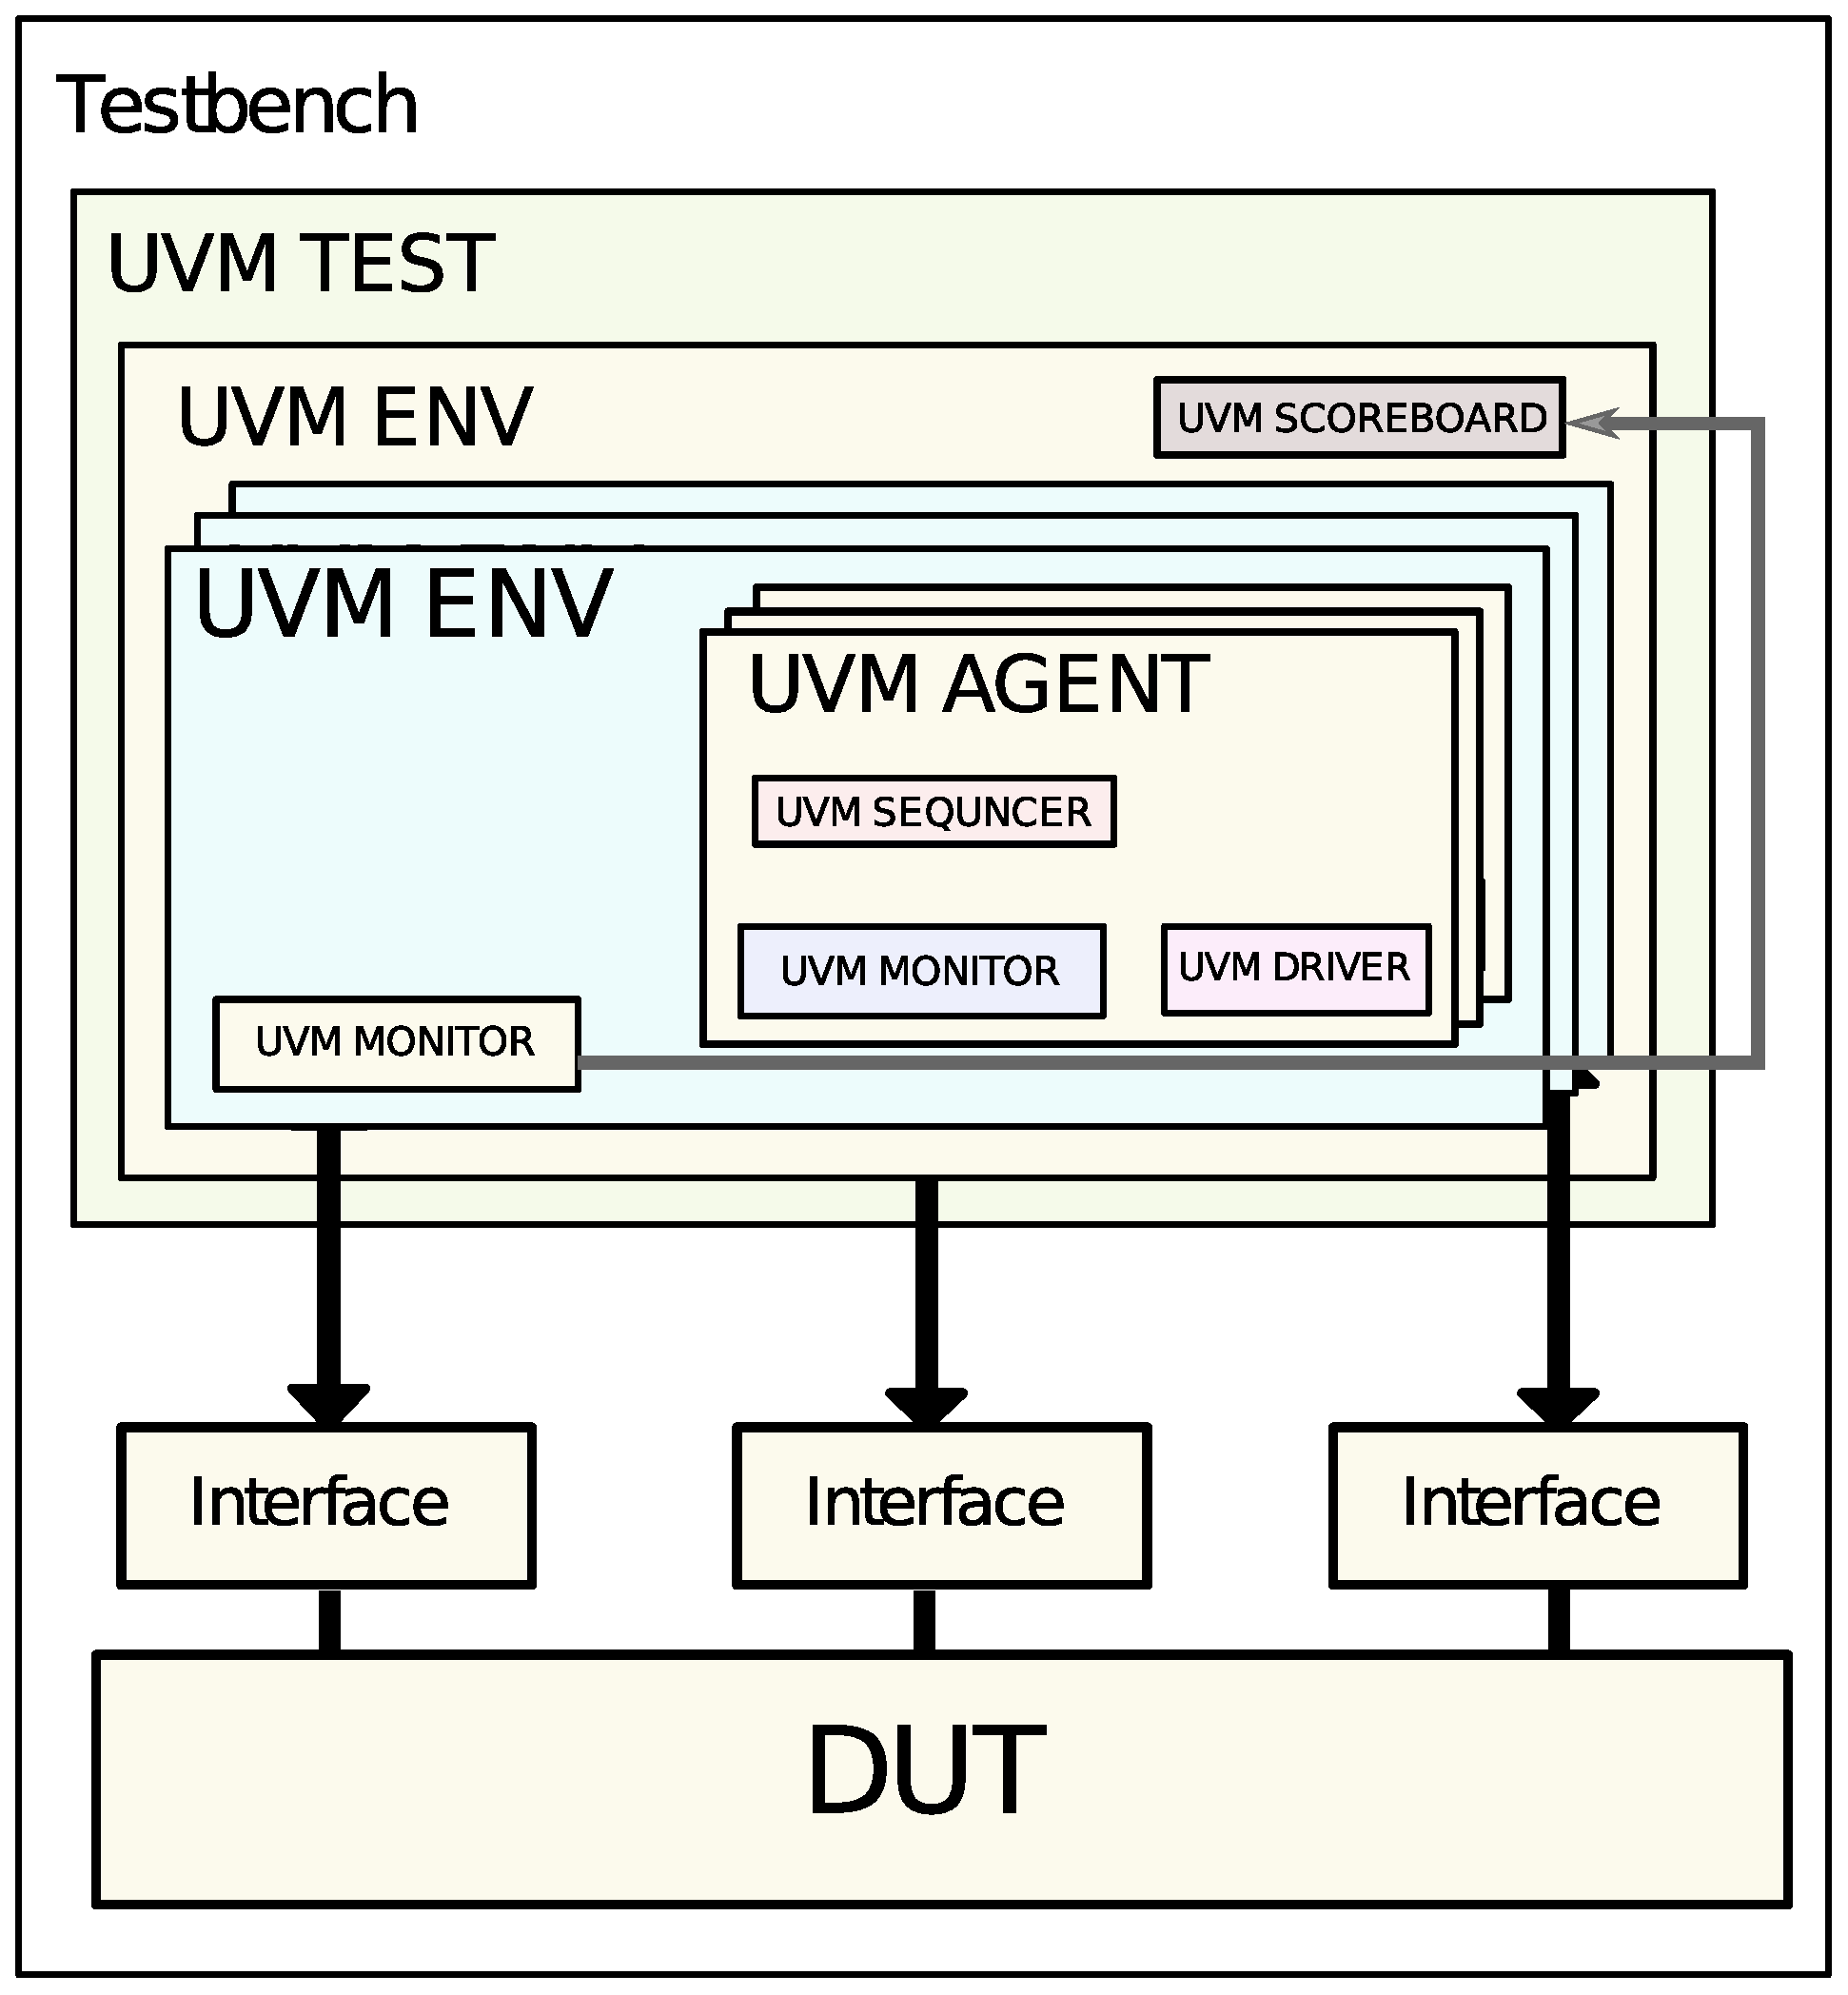
\includegraphics[width=0.5\linewidth]{pictures/UVM_testbench_architecture.eps}
\caption{UVM verification environment \cite{methodology20111}.}
\label{fig:UVMvenv}
\end{figure}

\subsection{UVM Overview}
The architecture of a UVM environment can be seen as an extension of a
traditional testbench. UVM testbenches are composed of shared components, like
drivers, scoreboards and monitors, and other classes that help create
standardized testbenches. UVCs compose a UVM testbench. UVCs are ready-to-use
configurable verification components intended for the functional verification of
protocols and modules \cite{methodology20111}. Each of the UVC components
follows a consistent architecture. The UVC interface is then applied to the DUT
to verify the protocol implementation and collect coverage information.

Figure \ref{fig:UVMvenv} represents a traditional UVM test environment. At the
core of the environment is the DUT or Device Under Test. The DUT interacts with
the UVM test by a series of stimuli generated as a sequence of data by a
umv\_sequencer component. In order to provide a high level of abstraction,
sequencers are unaware of the communication protocol. Their function is to
generate generic sequences of data and pass them to the umv\_driver block
responsible for handling the protocol's communication details and driving the
DUT pin toggling. The umv\_driver as a component is only responsible for
maintaining the communication with the device and feeding it data received from
the uvm\_sequencer.

The uvm\_monitor component monitors the validation of the DUT's response by
sampling the input and output stimuli sent and received by the DUT.
uvm\_monitors can be used to make predictions of the expected results and send
the prediction and result to another block called the uvm\_scoreboard. All these
components are the basis of a typical verification environment shared across all
the UVM testbenches. To increase the flexibility of each testbench, it is a best
practice to collect components like uvm\_sequencers, uvm\_drivers, and
uvm\_monitors inside an uvm\_agent class.

An uvm\_agent and a uvm\_scoreboard can then be incorporated into an uvm\_env
class. All these blocks are instantiated in the top-level block called
uvm\_test. The uvm\_test class is responsible for controlling all the blocks and
sub-blocks of the testbench. The described hierarchy allows a simplified control
of the verification environment and a higher degree of reconfigurability by
adding or removing specific blocks declared inside the uvm\_test class without
rewriting the whole testbench.


\subsubsection{UVM Classes}
OOP allows modeling the testbench with smaller components that can be easily
swapped and replaced without modifying the entire testbench. In UVM, all the
mentioned blocks are represented as objects derived from already existent
classes. A class tree of the essential UVM classes can be seen in the figure
\ref{fig:uvm:partial_tree}

\begin{figure}[htb]
\centering
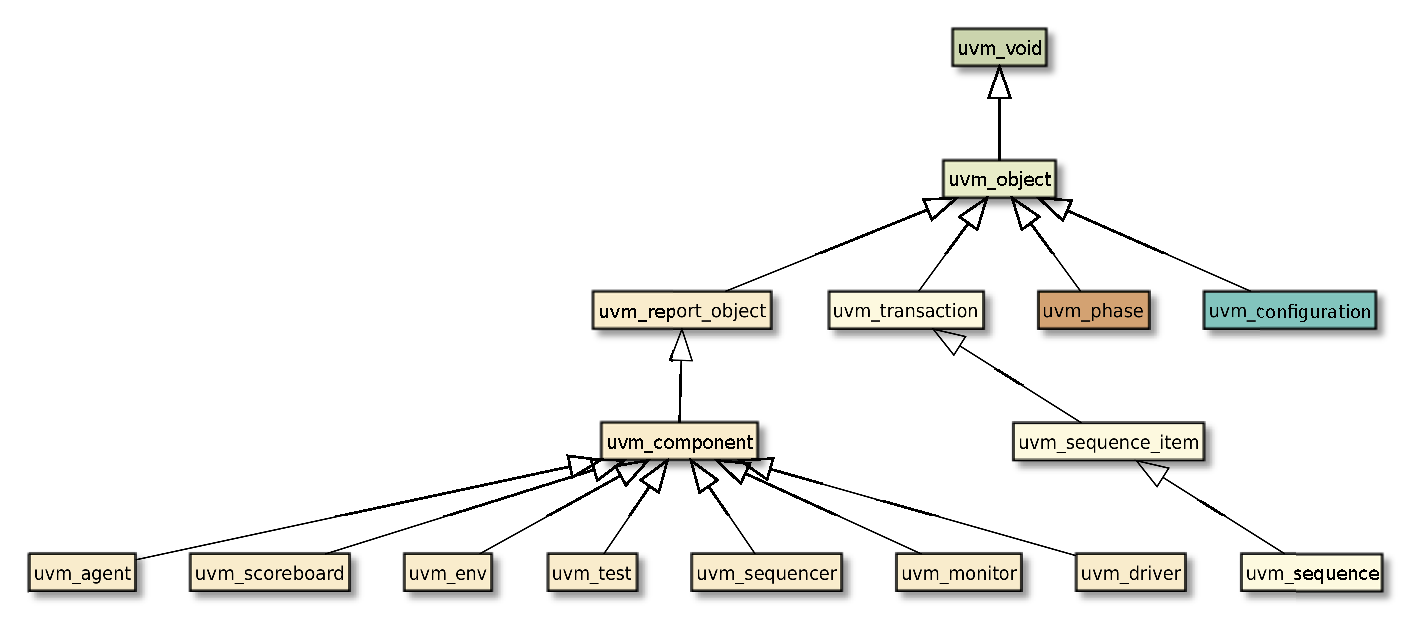
\includegraphics[width=\linewidth]{pictures/UVM_class_tree.eps}
\caption{Partial UVM class tree \cite{initiative94558universal}.}
\label{fig:uvm:partial_tree}
\end{figure}

\par In figure \ref{fig:uvm:partial_tree} are listed three new classes
uvm\_transaction, uvm\_sequence\_item and umv\_sequence. The classes are used to
encapsulate the data exchanged between the DUT and the environment. This data
will be stored in a class derived either from uvm\_sequence\_item or
uvm\_sequence. From the picture we can see that the classes in the UVM hierarchy
fall into two categories: data and components. The data class hierarchy derives
from uvm\_sequence\_item and component classes are derived from uvm\_component
and both have a common ancestor the uvm\_object. Component objects are created
at the beginning of the simulation (simulation time zero) while the UVM data
objects can be constructed at any time.

\par On top of different classes, UVM introduces the concept of phases. Each
component implements a set of callbacks executed in a specific ``phase" of the
simulation. The objects' callbacks are expected to be overwritten by the user to
initialize the object or perform a set of actions during a specific phase. The
UVM list of phases are build\_phase, connect\_phase,
end\_of\_elaboration\_phase, start\_of\_simulation\_phase, run\_phase,
extract\_phase, check\_phase, report\_phase, and final\_phase.


\par Given the high level of utilities function and methods introduced by the
UVM framework, the user is expected to implement a sustainable amount of methods
manually. For example, one of the most commonly manually implemented methods in
a user-defined component is the print method that prints the class's content. To
lower the burden of implementing most of the methods required, UVM introduces
the concept of UVM\_MACROS. UVM\_MACROS are a series of macros offered by the
framework meant to initialize and provide a default implementation for common
methods part of custom data structures defined by the user. UVM\_MACROS are
mostly needed because of the absence of reflective support by the SystemVerilog
language and are one of the most controversial feature of the UVM methodology
\cite{ bromley2013if, online:sysvreflections}.

\par For many verification engineers, verification is synonymous with
SystemVerilog plus UVM. In the verification domain, UVM became so pervasive that
vendors' tools are starting to integrate specific debug capabilities targeting
the UVM framework \cite{bromley2013if}. Even though this combination is widely
spread in the sector, the language's complexity combined with the framework led
to developers and engineers looking for other ways of functionally verifying
their models.

\section{Chisel / ChiselTester}
Chisel (Constructing Hardware In a Scala Embedded Language)
\cite{bachrach2012chisel} is an open-source Scala-based domain-specific language
for hardware generation. Using Scala as the donor language allows Chisel to
benefit from all its high-level programming utilities and functionalities. The
development of Chisel began in 2012 at University of California, Berkeley with
the intent of creating a new hardware description language that was flexible
enough to raise the level of abstraction offered by the traditional HDLs while
maintaining the ability to describe low-level hardware building blocks. In order
to be synthesizable, Chisel compiles down to Verilog. Contrary to most HDLs,
Chisel can be seen as a pure hardware construction language, and thus the
generated Verilog code is composed only of synthesizable constructors. Before
generating Verilog, Chisel is transformed into FIRRTL or Flexible Intermediate
Representation for RTL \cite{8203780}. Other than the possibility of generating
Verilog code from FIRRTL, this intermediate representation can be directly
simulated with Treadle \cite{online:treadle}, an open-source FIRRTL simulator
for quickly test hardware models described in Chisel.

Although Chisel is a relatively new hardware construction language compared to
SystemVerilog or other VHDL, it has already received much support from the
online community. Given its heritage from the software world, its community is
composed of hardware and software enthusiasts who push the development of the
language much faster than any other HDL so that, at the time of writing this
document, Chisel is at version 3.4.

To verify and test the model described in Chisel, hardware designers can use
ChiselTest. Built on top of the ScalaTest \cite{ScalaTest} library, ChiselTest
allows the simulation of the hardware model with Treadle. Being a software
library, ChiselTest enables concurrency using Scala threads with a set of API
that resemble the SystemVerilog concurrency one. Other than Treadle, ChiselTest
supports the Verilator \cite{verilator} simulator and offers a set of standard
APIs that can be used to implement different simulators as backends. ChiselTest
is still under development and is currently shipped separately from the Chisel
codebase.

\section{CoCoTB}
With the complexity and the verbosity of code needed by a SystemVerilog and UVM
verification environment, verification engineers started to research new ways of
functionally verifying new designs. One of them is CoCoTb or Coroutine based
Cosimulation TestBench environment for verifying VHDL/Verilog RTL using Python
\cite{online:cocotbpresentation}. CoCoTb leverages the broad adoption of the VPI
(Verilog Procedural Interface) by commercials and open-source simulators for
orchestrating the simulation of RTL designs. The VPI interface is standardized
by IEEE \cite{496013} and it defines a standard set of callbacks that enable an
interactive communication with the simulator during an RTL simulation. CoCoTb
provides an interactive simulation environment that hides the VPI interface's
complexity by providing a set of simple API to verify the model behavior as
shown in figure \ref{fig:cocotbsimenviron}. Many companies already started
switching away from UVM / SystemVerilog in favor of CoCoTb, given the large
availability of Python developers compared to UVM / SystemVerilog developers
\cite{online:cocotbpresentation}.

Furthermore, the extensibility of Python allows designers and verification
engineers, to quickly extends CoCoTb features. For example, the library
CoCoTb-Coverage provides a set of primitives for Coverage Driven Verification
\cite{cieplucha2016new}, while the library UVM-python \cite{online:uvmpython}
offers a porting of the full set of UVM classes and directives for CoCoTb. The
drawbacks of using CoCoTb for functional verification are mainly related to
using a verification language that is different from the design language. To use
CoCoTb for functional verification requires two different skill sets and, more
often than not, hardware designers are not familiar with Python and vice-versa
for Python developers. Another deficit is that this approach is highly coupled
with the VPI interface, which means that the environment is not easily portable
between different OS or OS versions.


\begin{figure}[htbp]
\centering
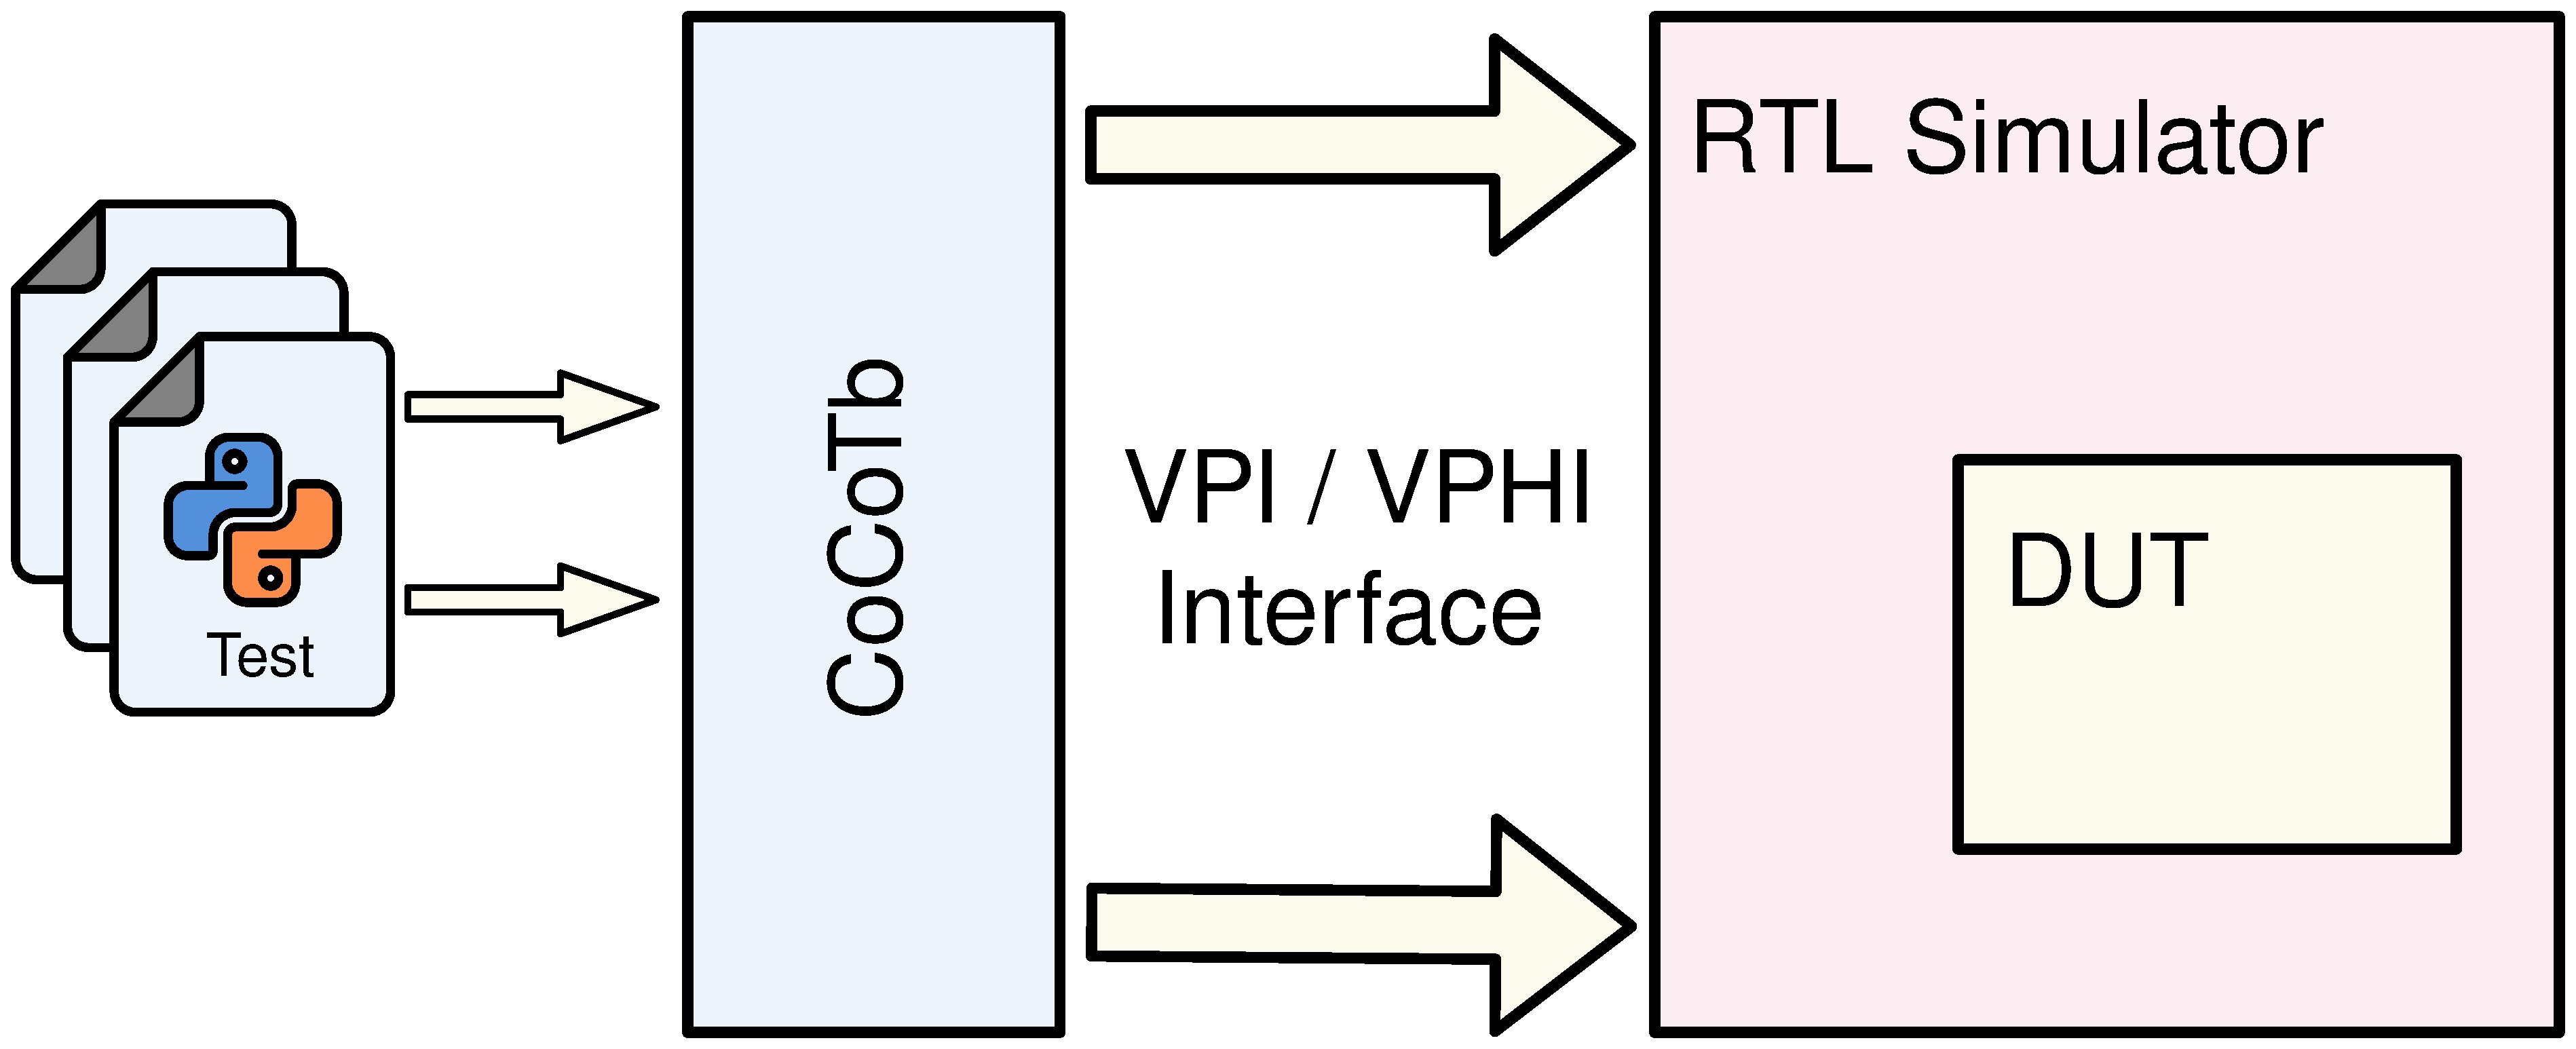
\includegraphics[width=0.6\linewidth]{pictures/CoCoTb_structure.eps}
\caption{CoCoTb simulation environment \cite{presentation:cerncocotb}.}
\label{fig:cocotbsimenviron}
\end{figure}
